\documentclass[xcolor={dvipsnames}]{beamer}
%\usepackage[utf8]{inputenc}
%\usetheme{Madrid}
\usetheme{CambridgeUS}
\usecolortheme{}

%-------------------------------------------------------------------------------
%          -Packages nécessaires pour écrire en Français et en UTF8-
%-------------------------------------------------------------------------------
\usepackage[utf8]{inputenc}
\usepackage[french]{babel}
\usepackage[T1]{fontenc}
\usepackage{lmodern}
\usepackage{textcomp}

%-------------------------------------------------------------------------------

%-------------------------------------------------------------------------------
%                          -Outils de mise en forme-
%-------------------------------------------------------------------------------
\usepackage{hyperref}
\hypersetup{pdfstartview=XYZ}
\usepackage{enumerate}
\usepackage{graphicx}
%\usepackage{multicol}
%\usepackage{tabularx}

%\usepackage{anysize} %%pour pouvoir mettre les marges qu'on veut
%\marginsize{2.5cm}{2.5cm}{2.5cm}{2.5cm}

\usepackage{indentfirst} %%pour que les premier paragraphes soient aussi indentés
\usepackage{verbatim}
%\usepackage[table]{xcolor}  
%\usepackage{multirow}
\usepackage{ulem}
%-------------------------------------------------------------------------------


%-------------------------------------------------------------------------------
%                  -Nécessaires pour écrire des mathématiques-
%-------------------------------------------------------------------------------
\usepackage{amsfonts}
\usepackage{amssymb}
\usepackage{amsmath}
\usepackage{amsthm}
\usepackage{tikz}
\usepackage{xlop}
\usepackage[output-decimal-marker={,}]{siunitx}
%-------------------------------------------------------------------------------

%-------------------------------------------------------------------------------
%                  -Nécessaires pour écrire des formules chimiquess-
%-------------------------------------------------------------------------------

\usepackage[version=4]{mhchem}

%-------------------------------------------------------------------------------
%                    - Mise en forme 
%-------------------------------------------------------------------------------

\newcommand{\bu}[1]{\underline{\textbf{#1}}}


\usepackage{ifthen}


\newcommand{\ifTrue}[2]{\ifthenelse{\equal{#1}{true}}{#2}{$\qquad \qquad$}}

\newcommand{\kword}[1]{\textcolor{red}{\underline{#1}}}


%-------------------------------------------------------------------------------



%-------------------------------------------------------------------------------
%                    - Racourcis d'écriture -
%-------------------------------------------------------------------------------

% Angles orientés (couples de vecteurs)
\newcommand{\aopp}[2]{(\vec{#1}, \vec{#2})} %Les deuc vecteurs sont positifs
\newcommand{\aopn}[2]{(\vec{#1}, -\vec{#2})} %Le second vecteur est négatif
\newcommand{\aonp}[2]{(-\vec{#1}, \vec{#2})} %Le premier vecteur est négatif
\newcommand{\aonn}[2]{(-\vec{#1}, -\vec{#2})} %Les deux vecteurs sont négatifs

%Ensembles mathématiques
\newcommand{\naturels}{\mathbb{N}} %Nombres naturels
\newcommand{\relatifs}{\mathbb{Z}} %Nombres relatifs
\newcommand{\rationnels}{\mathbb{Q}} %Nombres rationnels
\newcommand{\reels}{\mathbb{R}} %Nombres réels
\newcommand{\complexes}{\mathbb{C}} %Nombres complexes


%Intégration des parenthèses aux cosinus
\newcommand{\cosP}[1]{\cos\left(#1\right)}
\newcommand{\sinP}[1]{\sin\left(#1\right)}

%Fractions
\newcommand{\myfrac}[2]{{\LARGE $\frac{#1}{#2}$}}

%Vocabulaire courrant
\newcommand{\cad}{c'est-à-dire}

%Droites
\newcommand{\dte}[1]{$(#1)$}
\newcommand{\fig}[1]{figure $#1$}
\newcommand{\sym}{symétrique}
\newcommand{\syms}{symétriques}
\newcommand{\asym}{axe de symétrie}
\newcommand{\asyms}{axes de symétrie}
\newcommand{\seg}[1]{$[#1]$}
\newcommand{\monAngle}[1]{$\widehat{#1}$}
\newcommand{\bissec}{bissectrice}
\newcommand{\mediat}{médiatrice}
\newcommand{\ddte}[1]{$[#1)$}

%Figures
\newcommand{\para}{parallélogramme}
\newcommand{\paras}{parallélogrammes}
\newcommand{\myquad}{quadrilatère}
\newcommand{\myquads}{quadrilatères}
\newcommand{\co}{côtés opposés}
\newcommand{\diag}{diagonale}
\newcommand{\diags}{diagonales}
\newcommand{\supp}{supplémentaires}
\newcommand{\car}{carré}
\newcommand{\cars}{carrés}
\newcommand{\rect}{rectangle}
\newcommand{\rects}{rectangles}
\newcommand{\los}{losange}
\newcommand{\loss}{losanges}


\newcommand{\homo}{homothétie}
\newcommand{\homos}{homothéties}




%----------------------------------------------------
% Environnements de cours
%------------------------------------------------------



%\usepackage{../../../../pas-math}
\usepackage{../../../../moncours_beamer}





\graphicspath{{../img/}}
%Quelles sont les deux sortes de sources de lumière
\title{Exercice corrigé : la tension électrique}
%\author{O. FINOT}\institute{Collège S$^t$ Bernard}


\AtBeginSection[]
{
	\begin{frame}
		\frametitle{}
		\tableofcontents[currentsection, hideallsubsections]
	\end{frame} 

}


%\AtBeginSubsection[]
%{
%	\begin{frame}
%		\frametitle{Sommaire}
%		\tableofcontents[currentsection, currentsubsection]
%	\end{frame} 
%}

\begin{document}

\begin{frame}
  \titlepage 
\end{frame}


\begin{frame}
	\frametitle{\'Enoncé}
		
	Fatou a reçu en cadeau un manège miniature. Le jouet est alimenté par quatre piles de \num{1.5} $V$ qui fournissent une tension de 6 $V$. Un interrupteur permet d'allumer deux lampes qui éclairent les chevaux du manège et de commander en même temps le moteur qui fait tourner le manège.
	
	
	Fatou met en place les piles et les deux lampes fournies. Le moteur tourne normalement mais les lampes qui devaient éclairer la scène brillent très faiblement.\pause
	
	%Voici le schéma du circuit électrique du manège et les indications que Fatou trouve dans sa notice technique :
	
	\begin{columns}
		\begin{column}{0.4\textwidth}
			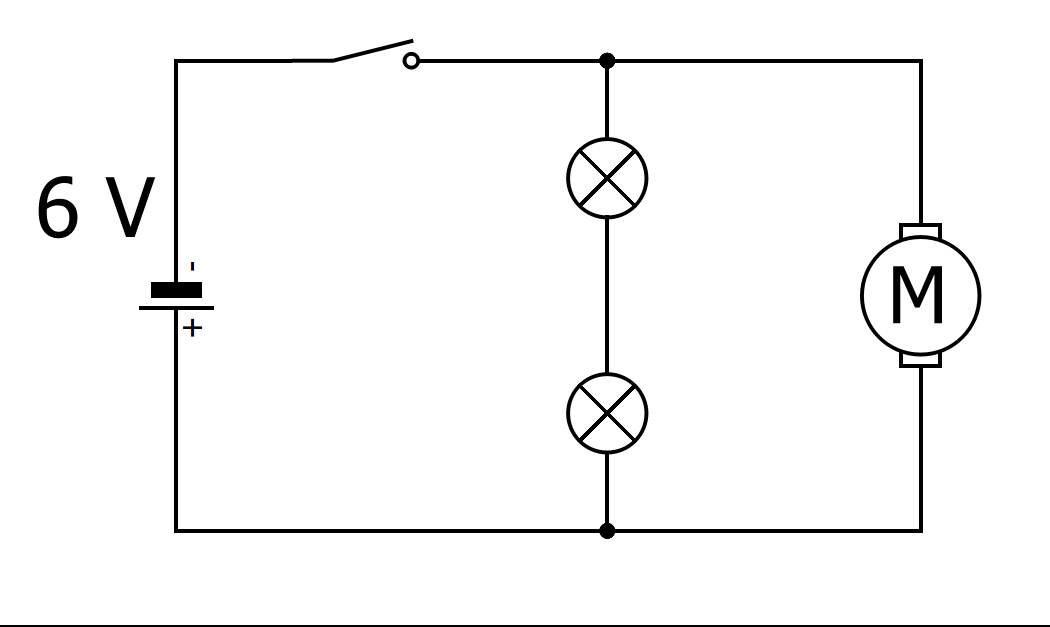
\includegraphics[scale=0.2]{../1_schema}
			
		\end{column}
	
		\begin{column}{0.6\textwidth}
			\begin{itemize}
				\item Tension nominale des lampes : 6 $V$
				\item Tension nominale du moteur : 6 $V$
			\end{itemize}		
			
		\end{column}
	\end{columns}	
\end{frame}

\begin{frame}
	\frametitle{Question 1}
	\begin{block}{}
		Quelle est la valeur de la tension $U_m$ aux bornes du moteur ?
	\end{block}

			
			\begin{columns}
				\begin{column}{0.4\textwidth}
					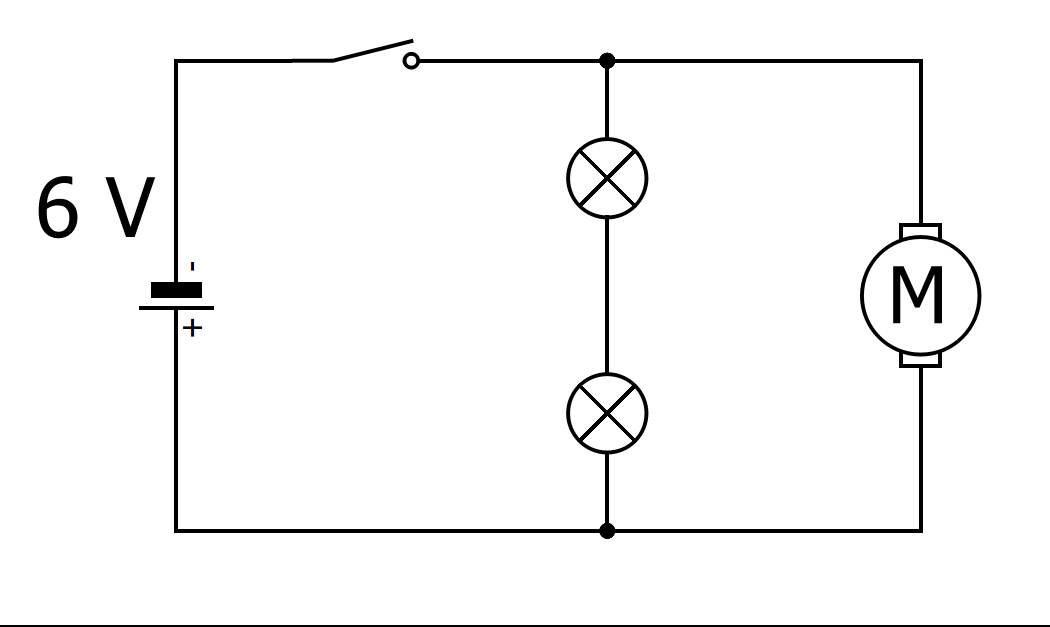
\includegraphics[scale=0.2]{../1_schema}
					
				\end{column}
				
				\begin{column}{0.6\textwidth}
					\begin{itemize}
						\item Tension nominale des lampes : 6 $V$
						\item Tension nominale du moteur : 6 $V$
					\end{itemize}		
					
				\end{column}
			\end{columns}

			\begin{block}<2->{Solution}
				Lorsque l'interrupteur est fermé il s'agit d'un circuit en dérivation qui comporte deux branches. Dans ce cas, la tension est la même aux bornes des deux branches. Donc la tension aux bornes du moteur est la même que celle aux bornes du générateur, 6 $V$.
			\end{block}
			

\end{frame}


\begin{frame}
\frametitle{Question 2}
\begin{block}{}
	Quelle est la valeur de la tension aux bornes de l'ensemble des deux lampes ?
\end{block}


\begin{columns}
	\begin{column}{0.4\textwidth}
		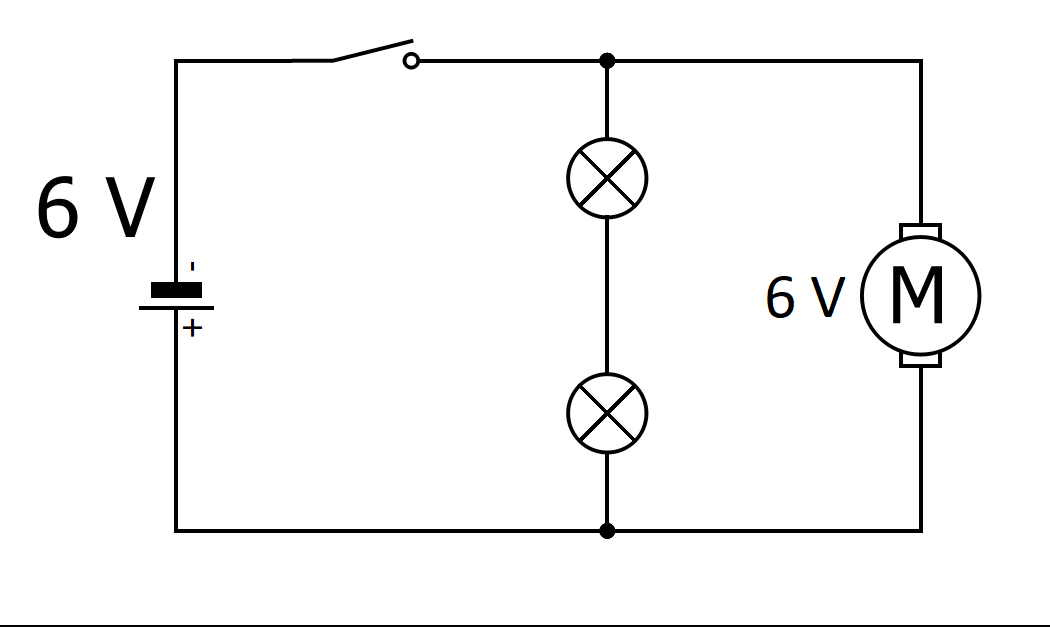
\includegraphics[scale=0.2]{../2_schema}
		
	\end{column}
	
	\begin{column}{0.6\textwidth}
		\begin{itemize}
			\item Tension nominale des lampes : 6 $V$
			\item Tension nominale du moteur : 6 $V$
		\end{itemize}		
		
	\end{column}
\end{columns}

\begin{block}<2->{Solution}
	Les deux lampes constituent la seconde branche, donc la tension à leur bornes est donc également 6 $V$.
\end{block}


\end{frame}

\begin{frame}
\frametitle{Question 3}
\begin{block}{}
	Calculer la tension aux bornes de chaque lampe (les lampes sont identiques).
\end{block}


\begin{columns}
	\begin{column}{0.4\textwidth}
		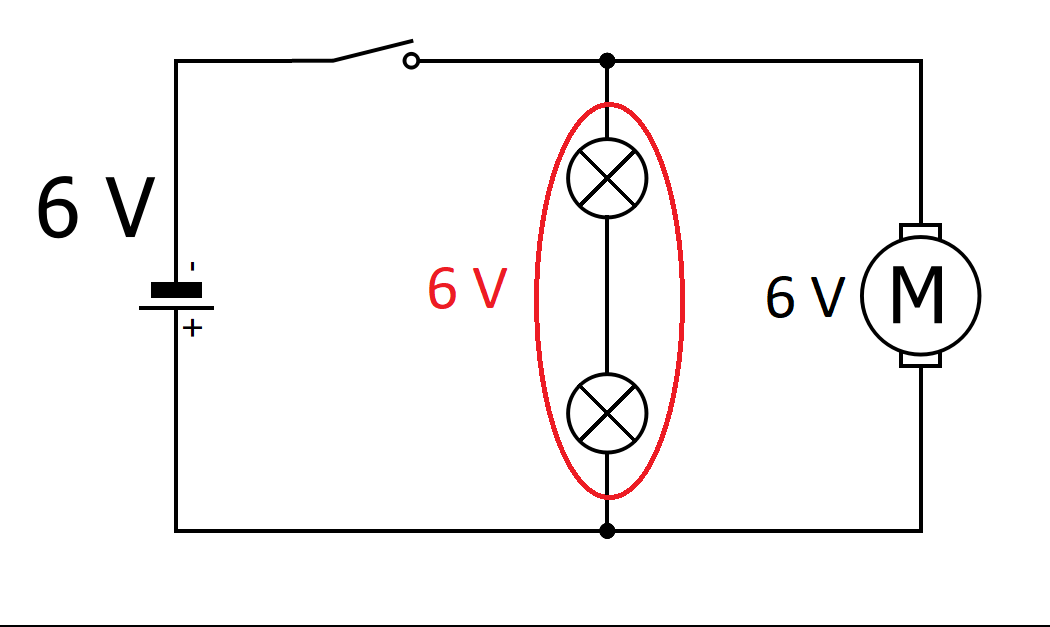
\includegraphics[scale=0.2]{../3_schema}
		
	\end{column}
	
	\begin{column}{0.6\textwidth}
		\begin{itemize}
			\item Tension nominale des lampes : 6 $V$
			\item Tension nominale du moteur : 6 $V$
		\end{itemize}		
		
	\end{column}
\end{columns}

\begin{block}<2->{Solution}
	Les deux lampes sont identiques et branchées en série l'une par rapport à l'autre. Les tensions aux bornes de dipôles branchés en série s'ajoutent. On a donc : $U_{L1} + U_{L2} = 6 V$ donc $U_{L1} = U_{L2} = 3 V$. La tension aux bornes de chaque lampe est 3 $V$.
\end{block}


\end{frame}


\begin{frame}
\frametitle{Question 4}
\begin{block}{}
	Expliquer pourquoi les deux lampes brillent faiblement.
\end{block}


\begin{columns}
	\begin{column}{0.4\textwidth}
		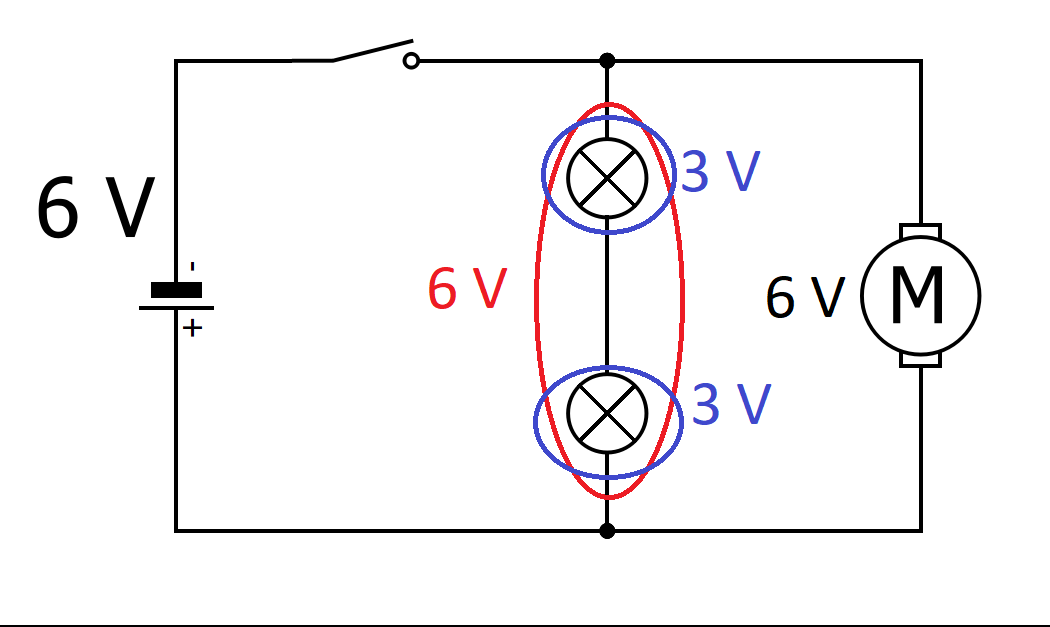
\includegraphics[scale=0.2]{../4_schema}
		
	\end{column}
	
	\begin{column}{0.6\textwidth}
		\begin{itemize}
			\item Tension nominale des lampes : 6 $V$
			\item Tension nominale du moteur : 6 $V$
		\end{itemize}		
		
	\end{column}
\end{columns}

\begin{block}<2->{Solution}
	La tension nominale des lampes est 6 $V$, donc chacune a besoin de 6 $V$ pour fonctionner correctement. Or elles ne reçoivent que 3 $V$, ce qui n'est pas suffisant pour qu'elles fonctionnent correctement.
\end{block}


\end{frame}
%\section{Reconnaître le dioxyde de carbone}
%
%\begin{frame}
%	\begin{myact}{4 page 127}
	\begin{enumerate}
		\item Le gaz prélevé dans la seringue a été extrait d'eau pétillante par déplacement d'eau.\pause
		\item Au début de l'expérience, la solution d'eau de chaux est incolore et transparente.\pause
		\item Après y avoir fait barboter le gaz l'eau de chaux s'est troublée.\pause
		\item Un précipité blanc s'est formé lors de cette expérience, donc le gaz dissous dans l'eau pétillante est du dioxyde de carbone.
	\end{enumerate}
\end{myact}
%\end{frame}
%
%
%\begin{frame}
%	\begin{mybilan}
	\begin{itemize}
		\item La masse d'un corps est \kw{proportionnelle} à son volume; \pause
		\item Le coefficient de proportionnalité est la \kw{masse volumique} (notée $\rho$);\pause
		\item \kw{Un litre d'eau} a une masse de \kw{1 kilogramme};\pause
		\item Une substance est \kw{plus dense} qu'une autre si, pour un même volume, sa masse est supérieure.		
	\end{itemize}
\end{mybilan}
%\end{frame}

\end{document}